\documentclass{standalone}
\usepackage{tikz}
\usepackage{float}
\usepackage{amsmath}
\usepackage{lmodern}
\usepackage{amssymb}
\usetikzlibrary{calc}
\usetikzlibrary{hobby}
\usepackage{nicefrac}
\usetikzlibrary{decorations.markings, decorations.pathreplacing}
\usetikzlibrary{patterns, patterns.meta}
\usetikzlibrary{shapes}
\usepackage{pgfplots}

\begin{document}


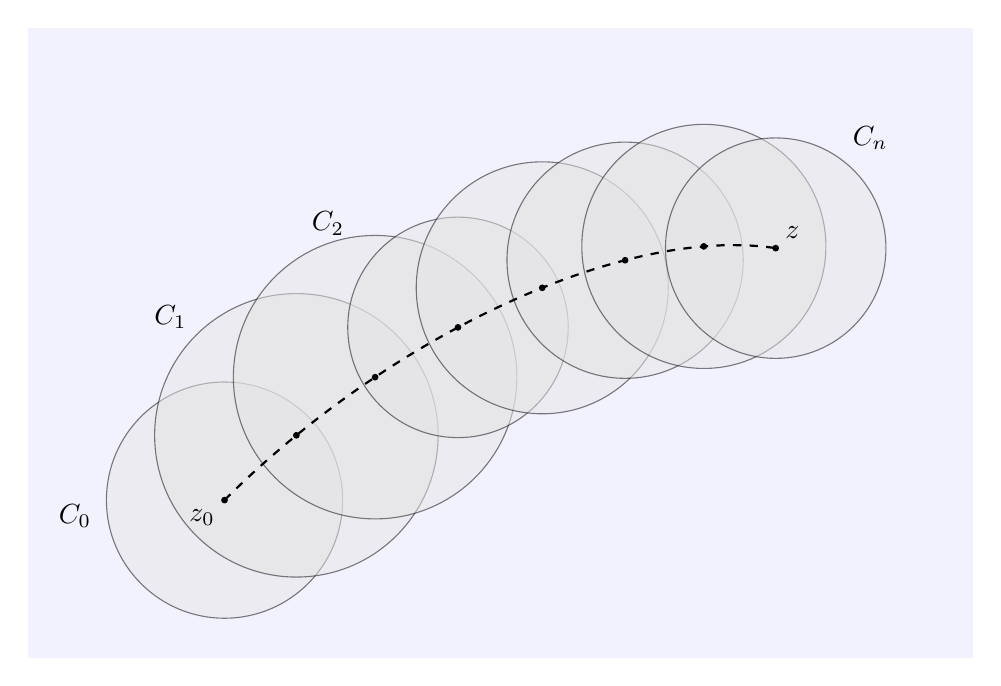
\begin{tikzpicture}

% Background for entire canvas
\fill[blue!5] (-2.5,-2) rectangle (9.5,6);
    
% Define 8 points along the curve (fractions of the total path length)
\foreach \i/\t in {0/z0, 1/z1, 2/z2, 3/z3, 4/z4, 5/z5, 6/z6, 7/z7} {
  \path 
    (0,0) .. controls (2,2) and (5,3.5) .. (7,3.2)
    coordinate[pos={\i/7}] (\t);
}

% Define radii and draw circles + midpoints
\foreach \i/\t/\r in {
  0/z0/1.5,
  1/z1/1.8,
  2/z2/1.8,
  3/z3/1.4,
  4/z4/1.6,
  5/z5/1.5,
  6/z6/1.55,
  7/z7/1.4
} {
  \filldraw[fill=gray!20, draw=black, opacity=0.5] (\t) circle (\r); % Circle
}

% Draw the midpoints (not in the previous loop, because circles will be drawn over it)
\foreach \i/\t in {
  0/z0,
  1/z1,
  2/z2,
  3/z3,
  4/z4,
  5/z5,
  6/z6,
  7/z7}{
  \filldraw[black] (\t) circle (1pt); % Midpoint
}

% Draw the smooth dashed curve using Bezier control points
\draw[dashed, thick]
  (0,0) .. controls (2,2) and (5,3.5) .. (7,3.2);
  
% Add labels
\node at (z0) [below left] {$z_0$};
\node at (z7) [above right] {$z$};
\node at ($(z0) + (-1.9,-0.2)$) {$C_0$};
\node at ($(z1) + (-1.6,1.5)$) {$C_1$};
\node at ($(z2) + (-0.6,1.95)$) {$C_2$};
\node at ($(z7) + (1.2,1.4)$) {$C_n$};

\end{tikzpicture}

\end{document}